\subsubsection{Acelerômetro piezoelétrico}

  As pás da turbina quando realizam rotações, criam vibrações no local onde elas estão girando. Como todas as outras partes
  estão interligadas, isso gera uma vibração em toda a estrutura. Essas vibrações são forças de variadas intensidades sendo
  geradas em vários pontos. Como qualquer estrutura mecânica, há um limite para as forças internas e externas agindo no sistema
  para que este não entre em colapso. A fim de se ter um controle maior sobre as vibrações causadas na estrutura para que
  estes eventos não causem sérios danos à turbina e seus componentes, serão utilizados acelerômetros como indicadores da
  vibração com o propósito de se monitorar os possíveis danos à estrutura.
  
  Os acelerômetros piezoelétricos (sensores de vibração) são componentes sensíveis a aplicações de forças neles. Funcionam da
  seguinte forma: as forças que são aplicadas a ele faz com que este se deforme, assim, produz cargas elétricas que são
  proporcionais às forças recebidas. Como a carga é proporcional à força e a massa é uma constante, a carga também é proporcional
  à aceleração. Dessa forma, estes componentes conseguem medir vibrações/acelerações (movimentação) de objetos relacionando com
  a proporção entre as forças aplicadas e as cargas elétricas produzidas \footnotemark.
  \footnotetext{Fonte: <https://br.omega.com/prodinfo/acelerometros.html>.}
  
  Foram feitas várias pesquisas a cerca de qual o melhor acelerômetro ser usado para o projeto, levando em conta preço, tipo do
  sensor, sensibilidade (mV/g). Dentre os encontrados, muitos estavam fora da faixa de sensibilidade adequada para o porte do
  projeto. Nos sites pololu.com \footnotemark \footnotetext{<https://www.pololu.com>} e
  sparkfun.com \footnotemark \footnotetext{<https://www.sparkfun.com>} não se encontrou acelerômetros piezoelétricos adequados, pois suas faixas
  de sensibilidade estão geralmente entre 3 g, 6 g, 12 g. Vale lembrar que 1 g = 9,8 $m/s^2$ (aceleração da gravidade). O sensor 
  escolhido foi decidido pela compatibilidade com a alta tolerância de impactos que ele resiste. Entretanto, no endereço 
  eletrônico \footnotemark \footnotetext{<https://www.imi-sensors.com/Products.aspx?m=339A30>} onde foi encontrado, o revendedor colocou o preço de \$ 0,00. A seguir se encontra uma imagem do
  sensor e logo após todas as especificações deste:
  
  \begin{figure}[!htbp]
    \centering
    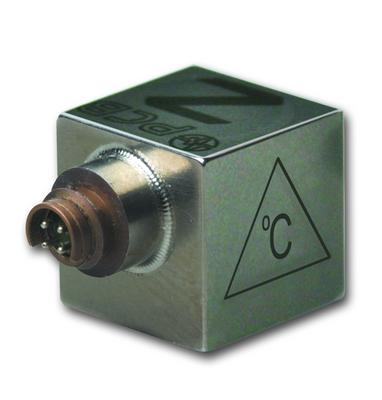
\includegraphics[scale=0.5]{editaveis/figuras/acelerometro}
    \caption[Acelerômetro para vibrações (\textit{Triaxial ICP accelerometer})]
    {Acelerômetro para vibrações (\textit{Triaxial ICP accelerometer}).}
    \label{acelerometro}
  \end{figure}
  
  A figura ~\ref{desempenho_acelerometro} ilustra o desempenho do acelerômetro. A figura ~\ref{param_eletrico_acelerometro} traz
   os parâmetros elétricos do acelerômetro. A figura ~\ref{ambiente_acelerometro} mostra os dados relativos ao ambiente.
  
  \begin{figure}[!htbp]
    \centering
    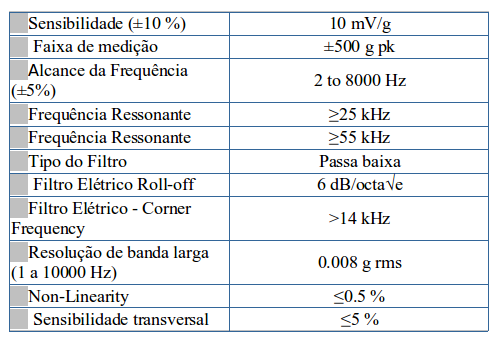
\includegraphics[scale=0.5]{editaveis/figuras/desempenho_acelerometro}
    \caption[Desempenho do acelerômetro]
    {Desempenho do acelerômetro.}
    \label{desempenho_acelerometro}
  \end{figure}
   
    \begin{figure}[!htbp]
	\centering
	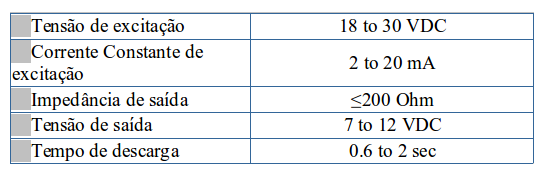
\includegraphics[scale=0.5]{editaveis/figuras/param_eletrico_acelerometro}
	\caption[Parâmetros elétricos do acelerômetro]{Parâmetros elétricos do acelerômetro.}
	\label{param_eletrico_acelerometro}
      \end{figure}
   
    \begin{figure}[!htbp]
      \centering
      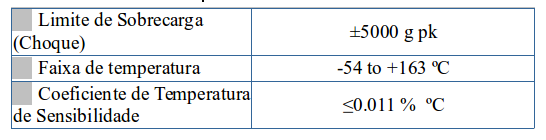
\includegraphics[scale=0.5]{editaveis/figuras/ambiente_acelerometro}
      \caption{Relativo ao ambiente.}
      \label{ambiente_acelerometro}
    \end{figure}